\documentclass[a4paper]{scrartcl}
\usepackage[ngerman]{babel}
\usepackage[utf8]{inputenc}
\usepackage{amsmath}
\usepackage{amssymb}
\usepackage{makeidx}
\makeindex{}
\usepackage{hyperref}
\usepackage{csquotes}
\usepackage{graphicx}

\usepackage[backend=biber,style=numeric]{biblatex}
\addbibresource{bibliography.bib}


%\renewcommand{\thesection}{Sitzung \Roman{section}: }
%\usepackage{titlesec}
%\titlelabel{Sitzung \thesection{} --- }
\title{Human Factors in Security and Privacy}
\author{\href{mailto:magnus.berendes@fau.de}{magnus.berendes@fau.de}}
\date{\today}
\begin{document}
\maketitle

\vfill
\begin{centering}
	Corrections, annotations and pull requests appreciated
	\\
\end{centering}


\newpage

\tableofcontents
\newpage
\printindex
\printbibliography
\newpage

\section{Introduction}
\begin{itemize}
	\item
		What is security?\index{Security}
		\begin{itemize}
			\item
				Protect the right thing in a right way (Anderson)
			\item
				Risk management: Trade-off between risk of attack and cost of protection
		\end{itemize}
	\item
		Defining Security:
		\begin{itemize}
			\item
				Goals: \textit{what} to protect

				Security properties of assets: CIA\index{CIA} (Confidentiality, Integrity, Availability)
			\item
				Threats: \textit{against what/whom} to protect
			\item
				Means: \textit{how} to protect

				Safeguards (attack prevention) and Countermeasures (detection and response)
		\end{itemize}
	\item
		Human Factors as Protection Means:
		\begin{itemize}
			\item
				Security management processes: policies, rules, decisions
			\item
				Usable security
			\item
				User education and training (apply with care!)
		\end{itemize}

	\item
		Security-questions to ask:
		\begin{itemize}
			\item
				System:
				\begin{itemize}
					\item
						Technical structure/organization
					\item
						Stakeholders: user types, service providers
					\item
						Assets: what should be protected?
				\end{itemize}
			\item
				Security goals? CIA?
			\item
				Threats/Attackers?
				\begin{itemize}
					\item
						Which threats are possible, probable, incur high losses?
					\item
						Incentives of the attackers?
					\item
						Resources/capabilities of the attackers?
				\end{itemize}
			\item
				Does the security measure protect against these attacks?
			\item
				If yes, is the protection \textit{effective}?
				\begin{itemize}
					\item
						Cost of protection vs. attack risk
					\item
						Are users capable of the required behavior?
				\end{itemize}
			\item
				Is it \textit{efficient}?
				\begin{itemize}
					\item
						Cost of protection (money, time, user effort (!) ) vs. attack risk
				\end{itemize}
		\end{itemize}
	\item

		\begin{figure}[ht]
			\centering
			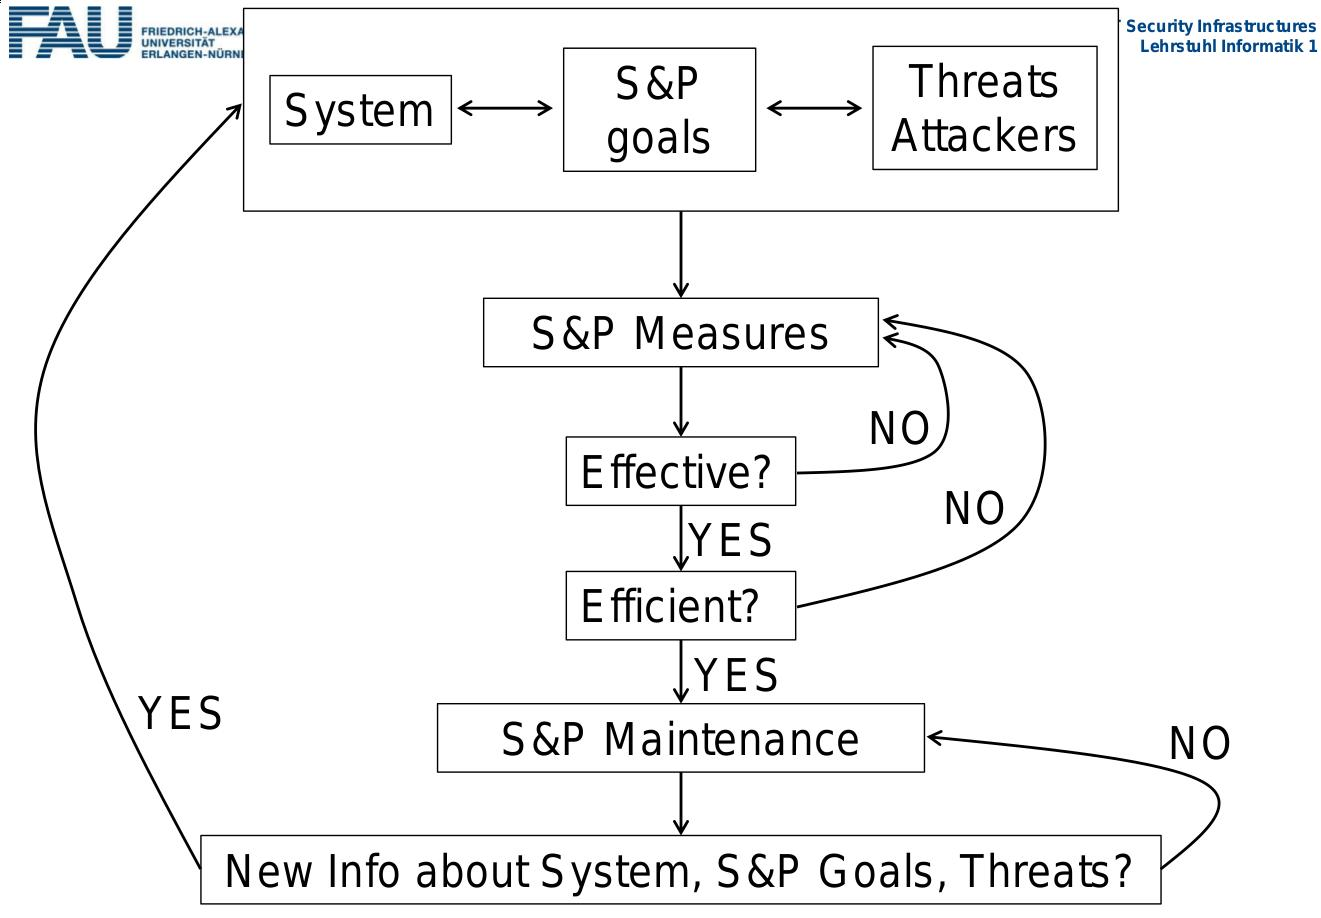
\includegraphics[
			width=0.8\textwidth]{security_process.jpg}
		\end{figure}

	\item
		Many S\&P measures offer bad trade-offs to the user: not much (subjective) gain of security, but a hassle
	\item
		\textit{Authorization}: \index{Authorization}
		\begin{itemize}
			\item
				Identification (e.g. login name)
			\item
				Plus authentication (e.g. password)
		\end{itemize}
\end{itemize}



\section{Passwords}
\begin{itemize}
	\item
		Security goals:
		\begin{itemize}
			\item
				Keep the bad guys out
			\item
				Don't lock me out!
		\end{itemize}
	\item
		Traditional password advice: strong (hard to guess), don't use it anywhere else, don't write it down, don't share it, change it often
	\item
		Do people follow this advice? No!
\end{itemize}
\subsection{Users are not the enemy}
\begin{itemize}
	\item
		\fullcite{usersenemy}
	\item
		Asked users about their password construction, frequency of use of different passwords, password recall
	\item
		Password diaries: write down all \enquote{happenings} around the password based authentication
	\item
		Findings:
		\begin{itemize}
			\item
				Users do not comply with policies
			\item
				but are not being wicked or stupid:
			\item
				They lack the right mental models of threats
			\item
				Password mechanisms lack user-centered design: not aligned with human memory capacities, not aligned with workflows (working together, delegating)
		\end{itemize}

		$\Rightarrow$ People chose weak passwords, reuse passwords, write them down, share them
	\item
		Mental Model \index{Mental Model}:
		\begin{itemize}
			\item
				Internal symbolic representation of external reality
			\item
				E.g. password=key model (how do i know if the website I'm logging into is real or fake? The key fits!)
			\item
				\enquote{Hackers cannot know the name of my cat, therefore that's a safe password}
		\end{itemize}
\end{itemize}

\subsection{A large-scale study of web password habits}
\begin{itemize}
	\item
		\fullcite{florenciolarge}
	\item
		544960 web clients, 3 months
	\item
		Windows Live Toolbar component with opt-in
	\item
		Report findings: websites, password compostion statistics (passwords were not transmitted), reuse, number of login attempts, time since last login
	\item
		Numnber of accounts per user: 25
	\item
		Each password shared across 4 different sites (avg)
	\item
		Passwords used per day: 8
	\item
		Mostly only lowercase letters \textit{unless forced to do otherwise}
\end{itemize}

\subsection{Passwords \& Human capabilities}
\begin{itemize}
	\item
		Why password logins fail:
		\begin{itemize}
			\item
				Failure to recall pssword

				Limited capacity of memory, decay over time, only unaided recall (no cues), items are non-meaningful, passwords are confused (items are similar and compete in memory), remember old password
			\item
				Typing errors

				no feedback on failure, needs to be 100\% correct
			\item
				Incorrect User ID
			\item
				User ID $\leftrightarrow$ password confusion
			\item
				Lock out after 3 attemps:

				Increasing to 10 tries decreases resets by 45\%
		\end{itemize}
	\item
		\fullcite{inglesanttrue}
		\begin{itemize}
			\item
				Data collection:  password diaries and interviews at two companies
			\item
				Conclusion very similar to \enquote{Users are not the enemy} from 1999 --- no positive changes after 10 years
		\end{itemize}
	\item
		\fullcite{florenciosecurity}
		\begin{itemize}
			\item
				Policies concentrate on forcing users to produce \enquote{strong} passwords
			\item
				Analysed \index{Minimal strength of password policies} minimal strength of password policies over 75 websites
			\item
				Minimal strength of a password policy: $N_{min} \log_2 C$

				$N_{min}$: minimal length, $C$: Character Space
			\item
				Analyses strength of the policy, not the password (strength of \enquote{password} is roughly the same as of \enquote{p4\$\$w0rd}, policy of the latter is much stronger)
		\end{itemize}
\end{itemize}

\end{document}
